%===============================================================================
% LaTeX sjabloon voor de bachelorproef toegepaste informatica aan HOGENT
% Meer info op https://github.com/HoGentTIN/latex-hogent-report
%===============================================================================

\documentclass[dutch,dit,thesis]{hogentreport}

% TODO:
% - If necessary, replace the option `dit`' with your own department!
%   Valid entries are dbo, dbt, dgz, dit, dlo, dog, dsa, soa
% - If you write your thesis in English (remark: only possible after getting
%   explicit approval!), remove the option "dutch," or replace with "english".

\usepackage{lipsum} % For blind text, can be removed after adding actual content

%% Pictures to include in the text can be put in the graphics/ folder
\graphicspath{{graphics/}}

%% For source code highlighting, requires pygments to be installed
%% Compile with the -shell-escape flag!
\usepackage[section]{minted}
%% If you compile with the make_thesis.{bat,sh} script, use the following
%% import instead:
%% \usepackage[section,outputdir=../output]{minted}
\usemintedstyle{solarized-light}
\definecolor{bg}{RGB}{253,246,227} %% Set the background color of the codeframe

%% Change this line to edit the line numbering style:
\renewcommand{\theFancyVerbLine}{\ttfamily\scriptsize\arabic{FancyVerbLine}}

%% Macro definition to load external java source files with \javacode{filename}:
\newmintedfile[javacode]{java}{
    bgcolor=bg,
    fontfamily=tt,
    linenos=true,
    numberblanklines=true,
    numbersep=5pt,
    gobble=0,
    framesep=2mm,
    funcnamehighlighting=true,
    tabsize=4,
    obeytabs=false,
    breaklines=true,
    mathescape=false
    samepage=false,
    showspaces=false,
    showtabs =false,
    texcl=false,
}

% Other packages not already included can be imported here

%%---------- Document metadata -------------------------------------------------
% TODO: Replace title, maybe!
\author{Lucca Van Veerdeghem}
\supervisor{Dhr. L. Smits}
\cosupervisor{Dhr. H. Kaymak}
\title[Onderzoek naar ontwikkelarchitecturen]%
    {Energie-efficiëntie in softwareontwikkeling}
\academicyear{\advance\year by -1 \the\year--\advance\year by 1 \the\year}
\examperiod{1}
\degreesought{\IfLanguageName{dutch}{Professionele bachelor in de toegepaste informatica}{Bachelor of applied computer science}}
\partialthesis{false} %% To display 'in partial fulfilment'
%\institution{Internshipcompany BVBA.}

%% Add global exceptions to the hyphenation here
\hyphenation{back-slash}

%% The bibliography (style and settings are  found in hogentthesis.cls)
\addbibresource{bachproef.bib}            %% Bibliography file
\addbibresource{../voorstel/voorstel.bib} %% Bibliography research proposal
\defbibheading{bibempty}{}

%% Prevent empty pages for right-handed chapter starts in twoside mode
\renewcommand{\cleardoublepage}{\clearpage}

\renewcommand{\arraystretch}{1.2}

%% Content starts here.
\begin{document}

%---------- Front matter -------------------------------------------------------

\frontmatter

\hypersetup{pageanchor=false} %% Disable page numbering references
%% Render a Dutch outer title page if the main language is English
\IfLanguageName{english}{%
    %% If necessary, information can be changed here
    \degreesought{Professionele Bachelor toegepaste informatica}%
    \begin{otherlanguage}{dutch}%
       \maketitle%
    \end{otherlanguage}%
}{}

%% Generates title page content
\maketitle
\hypersetup{pageanchor=true}

%%=============================================================================
%% Voorwoord
%%=============================================================================

\chapter*{\IfLanguageName{dutch}{Woord vooraf}{Preface}}%
\label{ch:voorwoord}

%% TODO:
%% Het voorwoord is het enige deel van de bachelorproef waar je vanuit je
%% eigen standpunt (``ik-vorm'') mag schrijven. Je kan hier bv. motiveren
%% waarom jij het onderwerp wil bespreken.
%% Vergeet ook niet te bedanken wie je geholpen/gesteund/... heeft

Met trots presenteer ik hierbij mijn bachelorproef, getiteld "Onderzoek naar vermindering van energieverbruik binnen softwareontwikkeling." Gedurende de afgelopen periode heb ik me verdiept in dit boeiende onderwerp, gedreven door mijn passie voor softwareontwikkeling en de voortdurende zoektocht naar optimalisatie ervan.\\

De keuze voor dit onderwerp kwam voort uit mijn interesse voor de technische aspecten van softwareontwikkeling en in het verbeteren van resource gebruik van software. In een tijd waarin duurzaamheid en energie-efficiëntie steeds belangrijker worden, is het verminderen van het energieverbruik binnen softwareontwikkeling een relevant en urgent vraagstuk.\\

Gedurende mijn onderzoekstraject heb ik het voorrecht gehad om te kunnen rekenen op de waardevolle begeleiding van mijn copromotor, Huzeyfe Kaymak. Ondanks zijn drukke agenda heeft hij tijd vrijgemaakt om mijn vragen te beantwoorden, mij te voorzien van waardevolle bijdragen en mij te begeleiden bij mijn onderzoek. Zijn expertise en toewijding hebben mijn onderzoek verrijkt en bijgedragen aan het succes ervan.\\

Tevens wil ik mijn dank uitspreken aan mijn familie, die mij gedurende dit hele proces heeft gesteund en van waardevolle feedback heeft voorzien. Hun aanmoediging en steun hebben mij gemotiveerd om door te zetten, zelfs tijdens de uitdagende momenten van dit onderzoeksavontuur.\\

Dit onderzoek zou niet mogelijk zijn geweest zonder de steun en inzet van deze mensen, en ik ben hen dan ook enorm dankbaar. Ik hoop dat dit onderzoek een waardevolle bijdrage levert aan het vakgebied van de softwareontwikkeling en bijdraagt aan het streven naar een duurzamere toekomst, alsook een aanstoot geeft tot verder onderzoek.\\

Met vriendelijke groet,

Lucca Van Veerdeghem
%%=============================================================================
%% Samenvatting
%%=============================================================================

% TODO: De "abstract" of samenvatting is een kernachtige (~ 1 blz. voor een
% thesis) synthese van het document.
%
% Een goede abstract biedt een kernachtig antwoord op volgende vragen:
%
% 1. Waarover gaat de bachelorproef?
% 2. Waarom heb je er over geschreven?
% 3. Hoe heb je het onderzoek uitgevoerd?
% 4. Wat waren de resultaten? Wat blijkt uit je onderzoek?
% 5. Wat betekenen je resultaten? Wat is de relevantie voor het werkveld?
%
% Daarom bestaat een abstract uit volgende componenten:
%
% - inleiding + kaderen thema
% - probleemstelling
% - (centrale) onderzoeksvraag
% - onderzoeksdoelstelling
% - methodologie
% - resultaten (beperk tot de belangrijkste, relevant voor de onderzoeksvraag)
% - conclusies, aanbevelingen, beperkingen
%
% LET OP! Een samenvatting is GEEN voorwoord!

%%---------- Nederlandse samenvatting -----------------------------------------
%
% TODO: Als je je bachelorproef in het Engels schrijft, moet je eerst een
% Nederlandse samenvatting invoegen. Haal daarvoor onderstaande code uit
% commentaar.
% Wie zijn bachelorproef in het Nederlands schrijft, kan dit negeren, de inhoud
% wordt niet in het document ingevoegd.

\IfLanguageName{english}{%
\selectlanguage{dutch}
\chapter*{Samenvatting}
\lipsum[1-4]
\selectlanguage{english}
}{}

%%---------- Samenvatting -----------------------------------------------------
% De samenvatting in de hoofdtaal van het document

\chapter*{\IfLanguageName{dutch}{Samenvatting}{Abstract}}
Dit onderzoek richtte zich op het analyseren het energieverbruik wanneer de ontwikkelarchitectuur van een applicatie veranderd wordt. De centrale onderzoeksvraag was: "Wat is de impact op energieverbruik bij een architecturale verandering van een applicatie?".\\

Om deze vraag te beantwoorden, werd een Proof of Concept (PoC) applicatie ontwikkelt in zowel een monolithische als een microservice versie. Beide versies werden gehost in een docker omgeving op een Ubuntu systeem en ondergingen diverse scenario's om het energieverbruik te meten. Specifieke methoden en controllers werden geïmplementeerd om gebruikers te laten inloggen en het verbruik van telefoonnummers te raadplegen, waardoor zowel resource intensieve als niet resource intensieve scenario’s werden gesimuleerd.\\

De testresultaten toonden aan dat de microservices aanzienlijk meer energie verbruiken dan monolithische applicaties, met een verschil van ongeveer 75\%. Dit verschil is evenredig aan de langere tijd die nodig is voor het uitvoeren van de scenario’s bij de microservices. Ondanks het hogere totale energieverbruik, hadden de microservices een lager gemiddeld wattverbruik vergeleken met de monolithische applicaties. Bovendien vertoonden monolithische applicaties grotere spreiding en variabiliteit in hun energieverbruik, wat wijst op inconsistente prestaties.\\

De analyse liet verder zien dat bij lage belasting het verschil in energieverbruik minimaal is, maar bij hoge belasting verbruiken microservices aanzienlijk meer tijd en dus ook meer energie, ondanks hun lagere gemiddelde wattverbruik. Dit kan verklaard worden door de afhankelijkheid van de microservices aan API-responstijden, terwijl monolithische applicaties direct kunnen reageren op inkomende requests.\\

Hoewel deze bevindingen relevant zijn voor ontwikkelaars en bedrijven die streven naar een vermindering van energieverbruik bij softwareontwikkeling, is er wel een belangrijke opmerking. Het onderzoek bevestigde dat een microservice architectuur op het gebied van energie besparen niet altijd de beste optie is, alhoewel ze een lager gemiddeld wattverbruik aanhouden. De conclusie van deze bachelorproef luidt daarom: `De architecturale verandering van een applicatie kan een negatieve impact hebben op het energieverbruik ervan.` Echter is dit niet het enige antwoord op deze onderzoeksvraag...\\

Toekomstig onderzoek zou zich kunnen richten op andere software ontwikkelarchitecturen, zoals serverless of event-driven architecturen, om een beter inzicht te krijgen in hoe verschillende architecturen het energieverbruik beïnvloeden. Dit zou kunnen bijdragen aan beter geïnformeerde beslissingen over architecturale keuzes en hun impact op energieverbruik.\\

Deze studie biedt waardevolle inzichten en draagt bij aan het vakgebied door de impact van architecturale keuzes op energieverbruik te belichten, wat belangrijk is voor de ontwikkeling van duurzame softwareoplossingen.

%---------- Inhoud, lijst figuren, ... -----------------------------------------

\tableofcontents

% In a list of figures, the complete caption will be included. To prevent this,
% ALWAYS add a short description in the caption!
%
%  \caption[short description]{elaborate description}
%
% If you do, only the short description will be used in the list of figures

\listoffigures

% If you included tables and/or source code listings, uncomment the appropriate
% lines.
%\listoftables
%\listoflistings

% Als je een lijst van afkortingen of termen wil toevoegen, dan hoort die
% hier thuis. Gebruik bijvoorbeeld de ``glossaries'' package.
% https://www.overleaf.com/learn/latex/Glossaries

%---------- Kern ---------------------------------------------------------------

\mainmatter{}

% De eerste hoofdstukken van een bachelorproef zijn meestal een inleiding op
% het onderwerp, literatuurstudie en verantwoording methodologie.
% Aarzel niet om een meer beschrijvende titel aan deze hoofdstukken te geven of
% om bijvoorbeeld de inleiding en/of stand van zaken over meerdere hoofdstukken
% te verspreiden!

%%=============================================================================
%% Inleiding
%%=============================================================================

\chapter{\IfLanguageName{dutch}{Inleiding}{Introduction}}%
\label{ch:inleiding}
De ICT-sector heeft in de afgelopen decennia een exponentiële groei in (complexe) toepassingen doorgemaakt, waardoor het een belangrijke rol speelt in onze moderne samenleving. De technologische vooruitgang verbergt een groeiend probleem: het toenemende energieverbruik van ICT-systemen. De huidige situatie duidt aan dat ongeveer 10\% van het wereldwijde elektriciteitsverbruik besteed wordt aan informaticasystemen, een percentage dat jaarlijks blijft stijgen \autocite{Gelenbe2023}.\\

Deze trend heeft de aandacht gevestigd op de dringende behoefte aan het verminderen van energieverbruik binnen de ICT-wereld. In dit kader is softwareontwikkeling een cruciale factor, omdat de gemaakte keuzes omtrent het ontwerpen en ontwikkelen van software een directe invloed hebben op het energieverbruik van de uiteindelijke systemen. Een voorbeeld hiervan is de opkomst van computed programmeertalen die ontwikkeling vereenvoudigen in vergelijking met de compiled talen, maar meer energie verbruiken \autocite{Manner2022}.\\

De poging tot het terugdringen van deze trend binnen softwareontwikkeling gaat verder dan enkel het minimaliseren van het energieverbruik. Het optimaal gebruik van resources binnen software is ook een belangrijke factor. Verschillende onderzoeken in het voorbije decennium hebben aangetoond dat het gebruik van gepaste ontwerp- en programmeerprincipes, zoals het toepassen van geschikte design patterns en het optimaliseren van datastructuren, een aanzienlijke invloed kan hebben op de hoeveelheid energie die een softwaretoepassing verbruikt. Elke use case is anders en kan niet via elk design pattern ontwikkeld worden.\\

Een voorbeeld van een niet geschikt design pattern voor een bepaalde use case zou het gebruik van een recursieve methode kunnen zijn voor het doorlopen van een grote dataset, waarbij elke recursieve oproep een nieuwe instantie van de methode creëert en mogelijks veel resources verbruikt. In plaats daarvan kan een iteratieve aanpak met een algoritme die minder resources verbruikt de voorkeur hebben om onnodig energieverbruik te vermijden.

%De inleiding moet de lezer net genoeg informatie verschaffen om het onderwerp te begrijpen en in te zien waarom de onderzoeksvraag de moeite waard is om te onderzoeken. In de inleiding ga je literatuurverwijzingen beperken, zodat de tekst vlot leesbaar blijft. Je kan de inleiding verder onderverdelen in secties als dit de tekst verduidelijkt. Zaken die aan bod kunnen komen in de inleiding~\autocite{Pollefliet2011}:

%\begin{itemize}
%  \item context, achtergrond
%  \item afbakenen van het onderwerp
%  \item verantwoording van het onderwerp, methodologie
%  \item probleemstelling
%  \item onderzoeksdoelstelling
%  \item onderzoeksvraag
%  \item \ldots
%\end{itemize}

\section{\IfLanguageName{dutch}{Probleemstelling}{Problem Statement}}%
\label{sec:probleemstelling}
\subsection{Davo Group NV, een bedrijfsschets}
Davo Group is een bedrijf dat begonnen is als eenmanszaak in 2009 en is momenteel uitgebouwd tot een bedrijf met meer dan 30 werknemers. Ze zijn een IT-integrator van performante, veilige datasnelwegen, complexe voice-oplossingen, VoIP-telefonie, Wi-Fi, netwerkbeveiliging, toegangscontrole, .... In maart 2024 trokken ze in in een nieuw, duurzaam, bedrijfscentrum te Drongen, genaamd In The Yard. Dit gebouw voldoet aan het WELL certificaat, dat duidt op energie- en waterbesparing, fossielvrij verwarmen, ...

\subsection{Probleem}
Davo Group ondernam al enkele stappen om als duurzamer bedrijf op de markt te staan. Nu kijken ze richting het Progress team, dat instaat voor de softwareontwikkeling binnen het bedrijf, om ook daar een poging te doen tot een duurzamere applicatieontwikkeling. Het huidige klantenportaal is uitgewerkt als een monoliet. Dit is een architectuur dat vrij verouderd is, alhoewel deze nog vaak gebruikt wordt in bedrijfsomgevingen. Dit wekte de vraag of een verandering in architectuur een positieve impact kan hebben op het energieverbruik. Daarvoor wensen ze te onderzoeken hoe verschillende ontwikkelarchitecturen, waaronder de monolithische architectuur, zich verhouden op het gebied van energieverbruik.
 
%Uit je probleemstelling moet duidelijk zijn dat je onderzoek een meerwaarde heeft voor een concrete doelgroep. De doelgroep moet goed gedefinieerd en afgelijnd zijn. Doelgroepen als ``bedrijven,'' ``KMO's'', systeembeheerders, enz.~zijn nog te vaag. Als je een lijstje kan maken van de personen/organisaties die een meerwaarde zullen vinden in deze bachelorproef (dit is eigenlijk je steekproefkader), dan is dat een indicatie dat de doelgroep goed gedefinieerd is. Dit kan een enkel bedrijf zijn of zelfs één persoon (je co-promotor/opdrachtgever).

\section{\IfLanguageName{dutch}{Onderzoeksvraag}{Research question}}%
\label{sec:onderzoeksvraag}
Om het probleem van Davo Group op te kunnen lossen is een onderzoek nodig die enkele architecturen vergelijkt tegenover de monolithische architectuur op vlak van energieverbruik voor een vooraf bepaalde use case. Dit brengt de vraag: `Wat is de impact op energieverbruik bij een architecturale verandering van een applicatie?'.

%Wees zo concreet mogelijk bij het formuleren van je onderzoeksvraag. Een onderzoeksvraag is trouwens iets waar nog niemand op dit moment een antwoord heeft (voor zover je kan nagaan). Het opzoeken van bestaande informatie (bv. ``welke tools bestaan er voor deze toepassing?'') is dus geen onderzoeksvraag. Je kan de onderzoeksvraag verder specifiëren in deelvragen. Bv.~als je onderzoek gaat over performantiemetingen, dan 

\section{\IfLanguageName{dutch}{Onderzoeksdoelstelling}{Research objective}}%
\label{sec:onderzoeksdoelstelling}
Het antwoord op de onderzoeksvraag is een eerste indicatie of softwareontwikkelarchitecturen een invloed heeft op het energieverbruik van een applicatie. Het onderzoek gebeurt aan de hand van een proof of concept waar een applicatie ontwikkeld wordt in 3 verschillende architecturen, met de monolithische architectuur er één van. 
%Wat is het beoogde resultaat van je bachelorproef? Wat zijn de criteria voor succes? Beschrijf die zo concreet mogelijk. Gaat het bv.\ om een proof-of-concept, een prototype, een verslag met aanbevelingen, een vergelijkende studie, enz.

\section{\IfLanguageName{dutch}{Opzet van deze bachelorproef}{Structure of this bachelor thesis}}%
\label{sec:opzet-bachelorproef}

% Het is gebruikelijk aan het einde van de inleiding een overzicht te
% geven van de opbouw van de rest van de tekst. Deze sectie bevat al een aanzet
% die je kan aanvullen/aanpassen in functie van je eigen tekst.

De rest van deze bachelorproef is als volgt opgebouwd:

In Hoofdstuk~\ref{ch:stand-van-zaken} wordt een overzicht gegeven van de stand van zaken binnen het onderzoeksdomein, op basis van een literatuurstudie.

In Hoofdstuk~\ref{ch:methodologie} wordt de methodologie toegelicht en worden de gebruikte onderzoekstechnieken besproken om een antwoord te kunnen formuleren op de onderzoeksvragen.

% TODO: Vul hier aan voor je eigen hoofstukken, één of twee zinnen per hoofdstuk
In Hoofdstuk~\ref{ch:short-list} wordt een lijst opgesteld met de gebruikte technologieën voor de proof of concept, ook wel de short list genoemd.

In Hoofdstuk~\ref{ch:opzet-poc} wordt de volledige opstelling van de proof of concept besproken. Hoe de applicaties zijn opgebouwd, welke methodes aanwezig zijn, de gebruikte data, ... wordt door dit hoofdstuk behandeld.

In Hoofdstuk~\ref{ch:test-poc} wordt er uitgebreid getest op de proof of concept. Resultaten zoals energieverbruik van elke applicatie worden hier opgenomen. 

In Hoofdstuk~\ref{ch:analyse-test-poc} worden de resultaten geanalyseerd om in Hoofdstuk~\ref{ch:conclusie} een conclusie te vormen.


Tenslotte, in Hoofdstuk~\ref{ch:conclusie}, wordt de conclusie gegeven en een antwoord geformuleerd op de onderzoeksvragen. Daarbij wordt ook een aanzet gegeven voor toekomstig onderzoek binnen dit domein.
\chapter{\IfLanguageName{dutch}{Stand van zaken}{State of the art}}%
\label{ch:stand-van-zaken}
In dit hoofdstuk wordt de huidige stand van zaken binnen het vakgebied van softwarearchitectuur en het verminderen van energieverbruik onderzocht. Allereerst wordt een overzicht gegeven van de meest recente ontwikkelingen en trends op het gebied van softwarearchitecturen. Vervolgens wordt de focus verlegd naar het belang van een lager energieverbruik binnen softwareontwikkeling, met een beschrijving van relevante concepten en benaderingen die worden gebruikt om energieverbruik te meten en te verminderen. Tenslotte wordt een overzicht gemaakt van de literatuurstudie om een stevige basis van begrip te leggen voor het verdere onderzoek binnen dit vakgebied.


\section{Ontwikkelarchitecturen}
De keuze van de juiste softwarearchitectuur is van cruciaal belang voor het succes van een softwareproject. Deze sectie bevat een inleiding tot verschillende ontwikkelarchitecturen, waaronder de monoliet architectuur en de microservices architectuur. Voor elke ontwikkelarchitectuur is er een oplijsting van hun kenmerken, voordelen en nadelen, alsook hun toepassingsgebied. 

\subsection{Wat is een architectuur}
Een software ontwikkelarchitectuur is een infrastructuur waarin applicatie componenten, die de functionele requirements voorzien, gespecificeerd, geïmplementeerd en uitgevoerd kunnen worden \autocite{Solms2012}. \textcite{Jaiswal2019} stelt dat een architectuur de blauwdruk is van een systeem, waarbij het complexiteit beheert en communicatie tussen componenten mogelijk maakt. Ze zijn als het ware een manier om herhalende problemen binnen software development aan te pakken door gebruik te maken van een fundamentele structuur, zijnde die blauwdruk \autocite{Dhaduk2020}.  Het levert een gestructureerde oplossing voor technische en operationele eisen, met aandacht voor kwaliteitskenmerken zoals prestaties en beveiliging. Elk van die architecturen heeft zijn voor en nadelen waardoor het belangrijk is om deze goed te vergelijken of ze in aanmerking komen voor de use case van de applicatie. Enkele voorbeelden van ontwikkelarchitecturen zijn: monolieten, microservices, event-driven architectuur, ...

\subsection{Opbouw architectuur}
Volgens \textcite{Solms2012} is een softwarearchitectuur opgebouwd uit 4 elementen:
\begin{itemize}
    \item Basis concepten en regels voor applicatie componenten die gebruikersfunctionaliteit voorzien;
    \item Architecturale componenten die technische zaken aanpakken;
    \item Manieren waarop er intern en/of extern met de applicatie gecommuniceerd wordt;
    \item Architecturale strategieën die de software kwaliteit beïnvloeden.
\end{itemize}


De basis concepten en regels zijn specifiek voor de bepaalde architectuur. Ze hebben 2 specifieke doelen, namelijk als extra documentatie om de architectuur beter te begrijpen en later makkelijk uitbreidingen toe te laten en te verifiëren of ze voldoen aan vooraf opgestelde regels en principes \autocite{Oussalah2013}. Verder hebben ze invloed op zowel de designfase als de implementatiefase.\\

De architecturale componenten zijn onderverdeeld in gebruikersinterface en structurele componenten \autocite{EDUCBA2023}. Deze laatste behandelen zaken zoals de functionaliteiten van de client en server, maar ook de database interactie. Verder is er ook een onderverdeling mogelijk in verschillende lagen, zoals aangetoond in figuur \ref{architectural_components_sota} die de architectuur van de applicatie iEnvironment toont. Er is de externe toegangslaag voor gebruikers die verbonden is met de gebruikersinterface laag. Die gaat dan op zijn beurt connectie maken naar de applicatielaag, datalaag en eventueel een externe toegangslaag waar de applicatiedata opgeslagen is. Elk van deze lagen is verantwoordelijk voor een bepaalde functionaliteit en zijn noodzakelijk om de volledige applicatie correct te laten verlopen.

\begin{figure}[ht]
    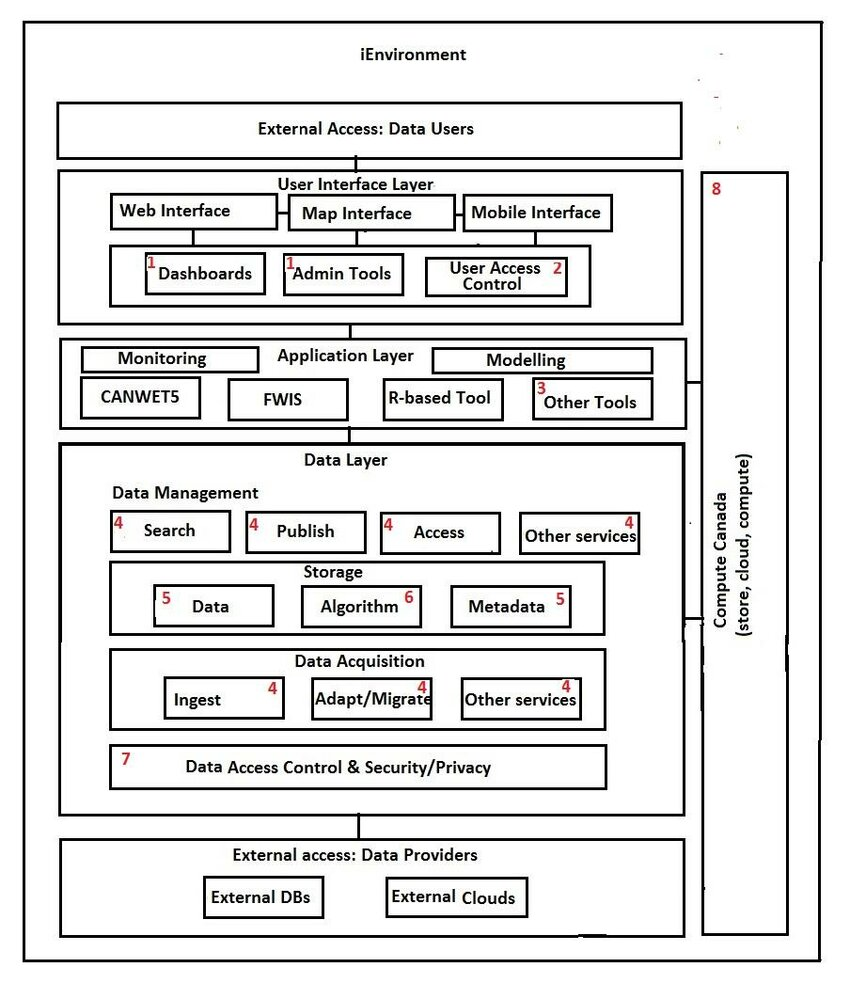
\includegraphics[scale=0.5]{architectural_components_sota}
    \centering
    \caption{Architecturale componenten iEnvironment \autocite{Alencar2018}}
    \label{architectural_components_sota}
\end{figure}

\bigskip

De manieren waarop communicatie mogelijk is met de applicatie moet ook duidelijk aangegeven zijn in de architectuur. De algemene regels is dat de toegang en integratie gespecificeerd is voor: functionaliteit binnen de architectuur, applicatie logica voor externe functionaliteiten en de architecturale componenten van de architectuur. Zo kan er bijvoorbeeld een web gebaseerde interface zijn voor menselijke gebruikers, terwijl systemen gebruik kunnen maken van web services zoals API's.\\

Als laatste zijn er de architecturale strategieën of ook wel tactieken genoemd. Ze zijn  ontwerpbeslissingen die het antwoord van de applicatie op een specifieke actie beïnvloeden dat belangrijk is voor bepaalde QA, quality attributes \autocite{Marquez2023}. Enkele beïnvloedbare QA door deze tactieken zijn aanpasbaarheid, afhankelijkheid, betrouwbaarheid, performantie, schaalbaarheid, ...

\subsection{Verschillende architecturen} \label{sota-title-architecturen}
\subsubsection{Monolithisch}
Alhoewel nog vaak voorkomend is de monolithische architectuur eerder verouderd waar modulariteit vaak niet aanwezig is\autocite{Megargel2020}. De user interface is rechtstreeks verbonden met business logica die doorverbonden staat met een database, zoals voorgesteld in figuur \ref{monolith_sota}. Elk onderdeel is gedefinieerd als een distinctieve architectuurlaag van een monoliet applicatie, respectievelijk de user interfacelaag, business logicalaag en databaselaag. \\

\begin{figure}[H]
    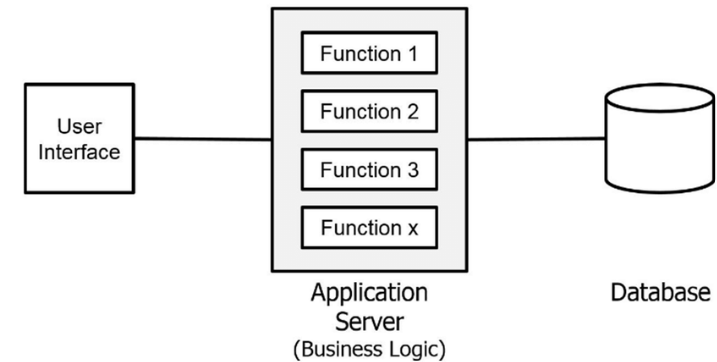
\includegraphics[scale=0.8]{monolith_sota}
    \centering
    \caption{Voorstelling monoliet \autocite{Megargel2020}}
    \label{monolith_sota}
\end{figure}


Het basis concept van deze architectuur is het centraal verzamelen van alle functies. Dit zorgt ervoor dat de applicatie 'simpel' is. Omdat alles centraal staat, is het makkelijk om een applicatie met deze architectuur te ontwikkelen, testen en deployen \autocite{Hou2023}. Een ander voordeel is het gemakkelijk onderhouden en debuggen van de applicatie. Verder zijn zoals eerder vermeld de architecturale componenten bij een monolithische architectuur duidelijk aanwezig. Deze structuur maakt het schalen van applicaties, zijnde optimaal houden van de applicatie bij een toegenomen gebruik ervan, moeilijk. Het overbelasten van 1 functie zal veel resources in beslag nemen, die eigenlijk gelijk verdeelt (moet) zijn onder alle functies. Het verticaal schalen is hier de oplossing voor, met het toevoegen van meer RAM bijvoorbeeld, maar is niet altijd een haalbare oplossing. Aangezien alle modules of functies van de applicatie op 1 server gedeployd zijn gebeuren alle operaties binnen hetzelfde proces en is er geen netwerk communicatie nodig om de interne werking te voorzien \autocite{Ozkaya2023}. 


\subsubsection{Microservices}
Microservices zijn een variant van de service-georiënteerde architectuur. Het bestaat uit een verzameling van kleine losse services die samenwerken tot de werking van een volledige applicatie \autocite{Megargel2020}. Een microservice omvat een business entiteit, bijvoorbeeld een product of een klant, of kan bepaalde activiteiten omvatten, zoals het plaatsen van een bestelling bij een webshop. Dit wordt visueel weergegeven in figuur \ref{microservice_sota} waar elk bolletje een microservice voorstelt die op zijn beurt een bepaalde functionaliteit van een business entiteit afhandelt.\\

\begin{figure}[H]
    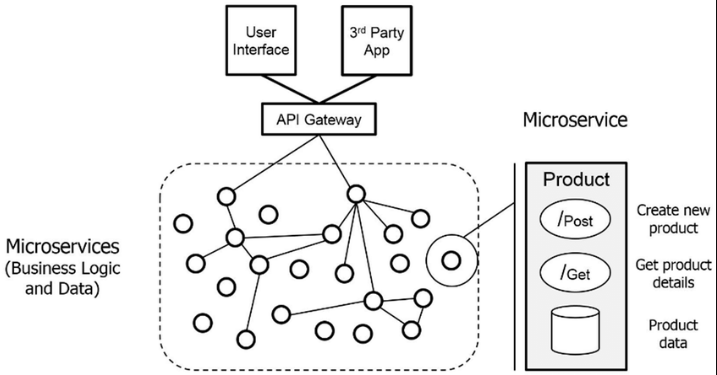
\includegraphics{microservice_sota}
    \caption{Voorstelling microservice architectuur \autocite{Megargel2020}}
    \label{microservice_sota}
\end{figure}

Het basisconcept bij deze architectuur is om elke functionaliteit zodanig op te splitsen dat elke business entiteit onafhankelijk kan functioneren. De architecturale componenten zijn hier, zoals voorgesteld in figuur \ref{microservice_sota}, een user interface of een applicatie van derden die verbonden is met een verzameling van microservices. De communicatie gebeurt via een API, waardoor zowel web applicaties als andere systemen gebruik kunnen maken van de beschikbaar gestelde functionaliteiten die de microservices bieden. Een van de gebruikte strategieën is het deployen naar een cloud omgeving die de applicatie automatisch extra resources kan toewijzen. Wanneer één service meer belast is dan de andere, krijgt deze automatisch meer resources toegewezen zonder dat de andere services hier een impact van ondervinden. Ook zorgt dit ervoor dat de applicatie grotendeels blijft werken wanneer een microservice (tijdelijk) niet beschikbaar is.

\subsubsection{Andere architecturen}
Er zijn nog vele andere architecturen, waaronder event driven architectuur, service georiënteerde architectuur, ... Ze verder opnoemen en in detail bespreken breidt de scope van deze bachelorproef te veel uit en wordt er enkel gefocust op de monoliet en de microservice architectuur. 

\subsection{Samengevat}
Samengevat wil dit zeggen dat een ontwikkelarchitectuur richtlijnen geeft hoe een applicatie ontwikkeld wordt. Het levert een structuur die de prestaties en beveiliging beïnvloeden. De 4 bouwdelen van een architectuur zorgen ervoor dat een applicatie gemakkelijk uitbreidbaar is, logisch is opgebouwd, bereikbaar is zowel voor mens als systemen en voldoet aan kwaliteitseisen.



\section{Energieverbruik van software}
Deze sectie verduidelijkt de definitie van energie-efficiëntie, alsook hoe software energie verbruikt. De verschillende benaderingen en technieken voor het meten en verminderen van energieverbruik zijn ook getackeld in dit hoofdstuk, waaronder optimalisatie van code.

\subsection{Wat is energie-efficiëntie}
Energie-efficiëntie is een generieke, niet-meetbare term \autocite{Patterson1996}. Het is wel een vergelijkbare term, in die zin dat men kan vergelijken hoeveel energie eenzelfde service of bruikbare output verbruikt in verschillende situaties. Het wordt vaak gedefinieerd als de ratio 
$\frac{\text{Bruikbare output}}{\text{Energie input}}$ . Dit kan gebruikt worden om het verschil in energieverbruik aan te tonen.

\subsection{Energieverbruik van software}
Het energieverbruik van software ligt nauw samen met de performantie ervan. Voor beiden worden de resources gemonitord, echter wordt andere data verzameld. Voor energieverbruik gaat het niet om in welke mate de applicatie resource gebruikt, maar eerder hoeveel energie ze dus verbruiken \autocite{Kor2015}. Het meten van energieverbruik is niet een eenmalige taak, maar gebeurt best meerdere keren over een bepaald scenario. Dit vormt een beter beeld over het effectieve energieverbruik van een applicatie in verschillende situaties, zoals mogelijke achtergrondprocessen dat eventueel een impact kunnen hebben.

\subsection{Link met programmeertalen}
Volgens \textcite{Jain2024} kan software in 2 manieren verdeeld worden waarop een applicatie vertaald wordt naar machine taal. Er is compiled language en interpreted language. Compiled gaat de volledige code voor het opstarten van het programma in zijn geheel compileren. Dit leidt tot een efficiëntere applicatie omdat de vertaling van code naar machine taal al gebeurd is. De interpreted language werkt op een hele andere manier. Hier wordt code lijn per lijn vertaald en uitgevoerd. Dit zorgt er dan voor dat de applicatie flexibeler is, met als nadeel dat de uitvoeringstijd vertraagd is.\\

Zo blijkt ook uit onderzoek van \textcite{Pereira2017} dat de keuze van programmeertaal een grote impact kan hebben op het energieverbruik van de applicatie. Zo blijkt uit figuur \ref{verbruik_taal_sota} dat C\footnote{https://www.cprogramming.com/}, een compiled language, de meest energiezuinige taal is en Perl\footnote{https://www.perl.org/}, een interpreted taal, het meeste energie verbruikt, namelijk tot wel 80 keer zoveel als C voor het runnen van eenzelfde applicatie. \\

\begin{figure}[H]
    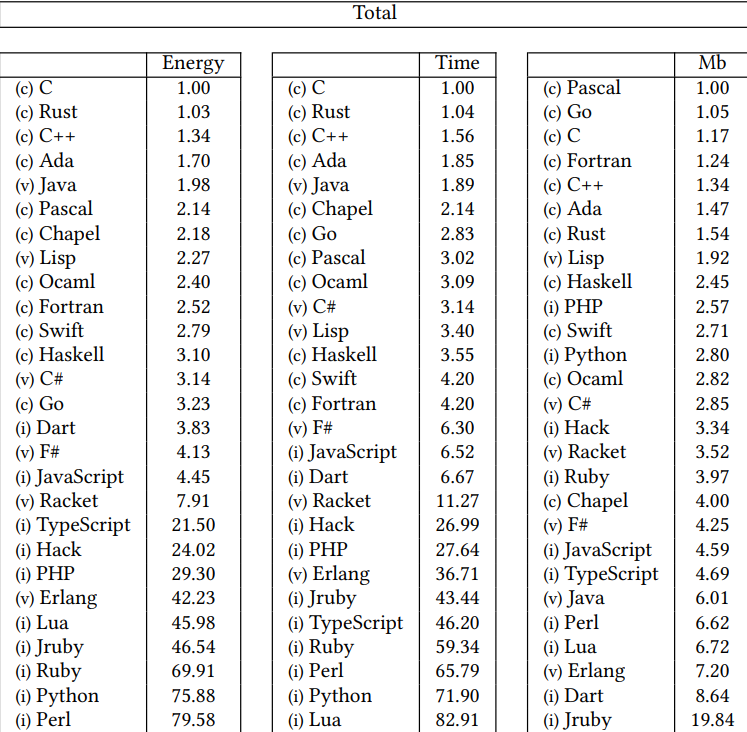
\includegraphics[scale=0.5]{verbruik_taal_sota}
    \centering
    \caption{Genormaliseerd energieverbruik, uitvoeringstijd en geheugengebruik van 1 scenario \autocite{Pereira2017}}
    
    \label{verbruik_taal_sota}
\end{figure}


\subsection{Link met programmeerprincipes}
Bij het ontwikkelen van programma's is de eindfunctionaliteit vaak vastgelegd. Het programma moet namelijk één of meerdere taken kunnen uitvoeren. Echter is het zo dat het niet vastligt hoe de ontwikkeling gebeurd. Om één bepaalde uitkomst te bekomen zijn er meerdere manieren om dit te verwezenlijken. Als verschillende programmeurs zelfstandig werken aan eenzelfde probleem, zal er zelden 100\% gelijke code voorkomen. Dit komt door de eigen stijl/manier van ontwikkelen.\\

In het onderzoek van \textcite{Hassan2017} wordt aangetoond dat een verschillende programmeerstijl impact kan hebben op het energieverbruik van een applicatie. Zo is er in figuur \ref{3_coding_styles_sota} een selection sort geprogrammeerd op 3 manieren. De eerste manier sorteert eerst de array en zal eenmaal gesorteerd de array uitschrijven naar de console. In de tweede manier zal tijdens het sorteren het algoritme de gesorteerde elementen al uitschrijven naar de console. Als laatste manier houdt men een zelfde werkwijze aan als de eerste manier, maar last men om de 500 items een pauze om de processor even te stoppen en na te gaan of een sleep operatie invloed heeft op het energieverbruik. De resultaten zijn beschikbaar in figuur \ref{energy_consumption_situations_sota}. Hieruit kan er besloten worden dat elke manier verschilt in energieverbruik. Dit is echter niet het enige wat deze resultaten aanduiden. De compilers waarop deze testen uitgevoerd werden hebben duidelijk ook een impact op het energieverbruik.\\

\bigskip

\begin{figure}[H]
    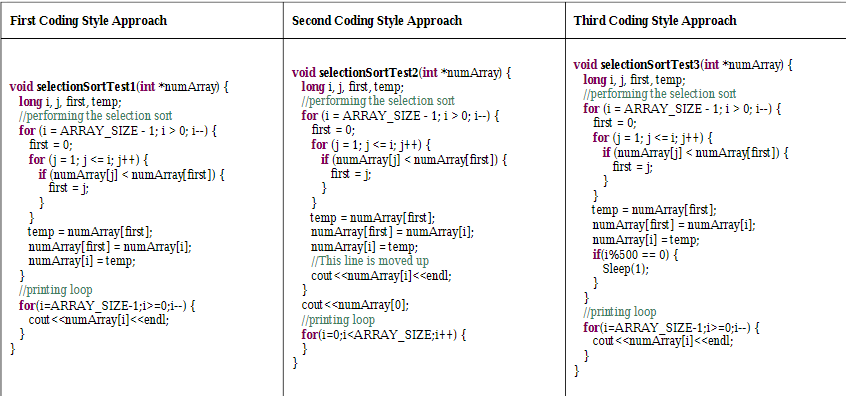
\includegraphics[scale=0.8]{3_coding_styles_sota}
    \centering
    \caption{3 manieren voor een selection sort \autocite{Hassan2017}}
    \label{3_coding_styles_sota}
\end{figure}

\begin{figure}[H]
    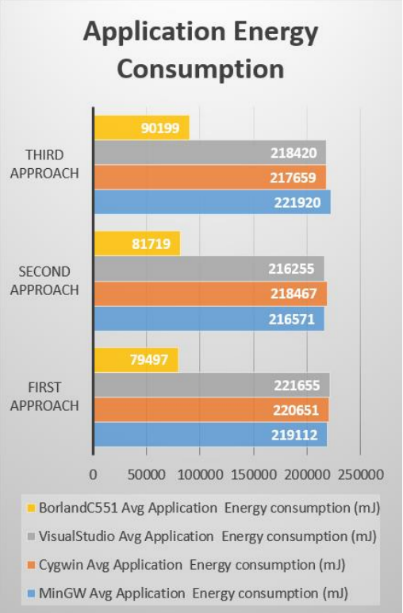
\includegraphics[scale=0.8]{energy_consumption_situations_sota}
    \centering
    \caption[Energieverbruik tussen programmeerstijlen]{Energieverbruik tussen verschillende programmeerstijlen in verschillende compilers \autocite{Hassan2017}}
    \label{energy_consumption_situations_sota}
\end{figure}



Ook datatypes spelen een rol in het energieverbruik van software. Gegevens opslaan in een datatype dat meer plaats inneemt in het geheugen of extra processing power nodig heeft leidt tot een hoger energieverbruik \autocite{Dutta2023}. Zo wordt in figuur \ref{energy_consumption_data_types_sota}, waar numerieke datatypes vergeleken worden, aangetoond dat er tot net geen 50\% energie bespaard kan worden op basis van het datatype. Deze situatie is niet altijd haalbaar, aangezien niet elk van deze datatypes geschikt is voor eenzelfde use case. 

\bigskip

Wat echter wel altijd haalbaar is, is wanneer een string, een datatype dat tekst bevat, voorgesteld moet worden. Het gebruik maken van een StringBuilder, een ingebouwde klasse die string operaties kan uitvoeren, verbruikt nagenoeg geen energie. Wanneer de gewone String klasse gebruikt wordt, verbruikt dit duizenden keren meer energie dan de StringBuilder. Dit fenomeen wordt aangetoond in figuur \ref{energy_consumption_string_sota}. 

\bigskip


\begin{figure}[H]
    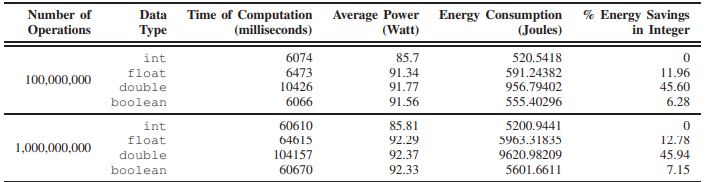
\includegraphics{energy_consumption_data_types_sota}
    \caption[Energieverbruik numerieke datatypes]{Vergelijken van energieverbruik bij numerieke datatypes \autocite{Dutta2023}}
    \label{energy_consumption_data_types_sota}
\end{figure}


\begin{figure}[H]
    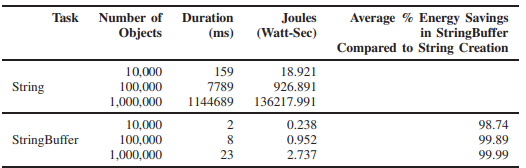
\includegraphics{energy_consumption_string_sota}
    \centering
    \caption[Energieverbruik string voorstelling]{Vergelijken van energieverbruik bij voorstellen van string values \autocite{Dutta2023}}
    \label{energy_consumption_string_sota}

\end{figure}


\subsection{Link met performantie}
Volgens \textcite{Lubomski2020} zijn de 3 karakteristieken die performantie bepalen responstijd, doorvoer van data en gebruik van resources. Ze beïnvloeden elkaar, bijvoorbeeld een trage doorvoer van data leidt tot een lage responstijd. Een performante applicatie probeert te streven naar de beste combinatie van de 3. Dit is dan een hoge datadoorvoer met een laag resource gebruik en een lage responstijd. 

\bigskip

Het karakteristiek dat inspeelt op energieverbruik van software is het resource gebruik. Hieronder valt CPU-, RAM-, disk- en netwerkgebruik. Dit wordt bevestigd door figuur \ref{cpu_usage_sota}, waar een hoger CPU-gebruik gelijk staat aan een hoger energieverbruik.\\



\begin{figure}[h!]
    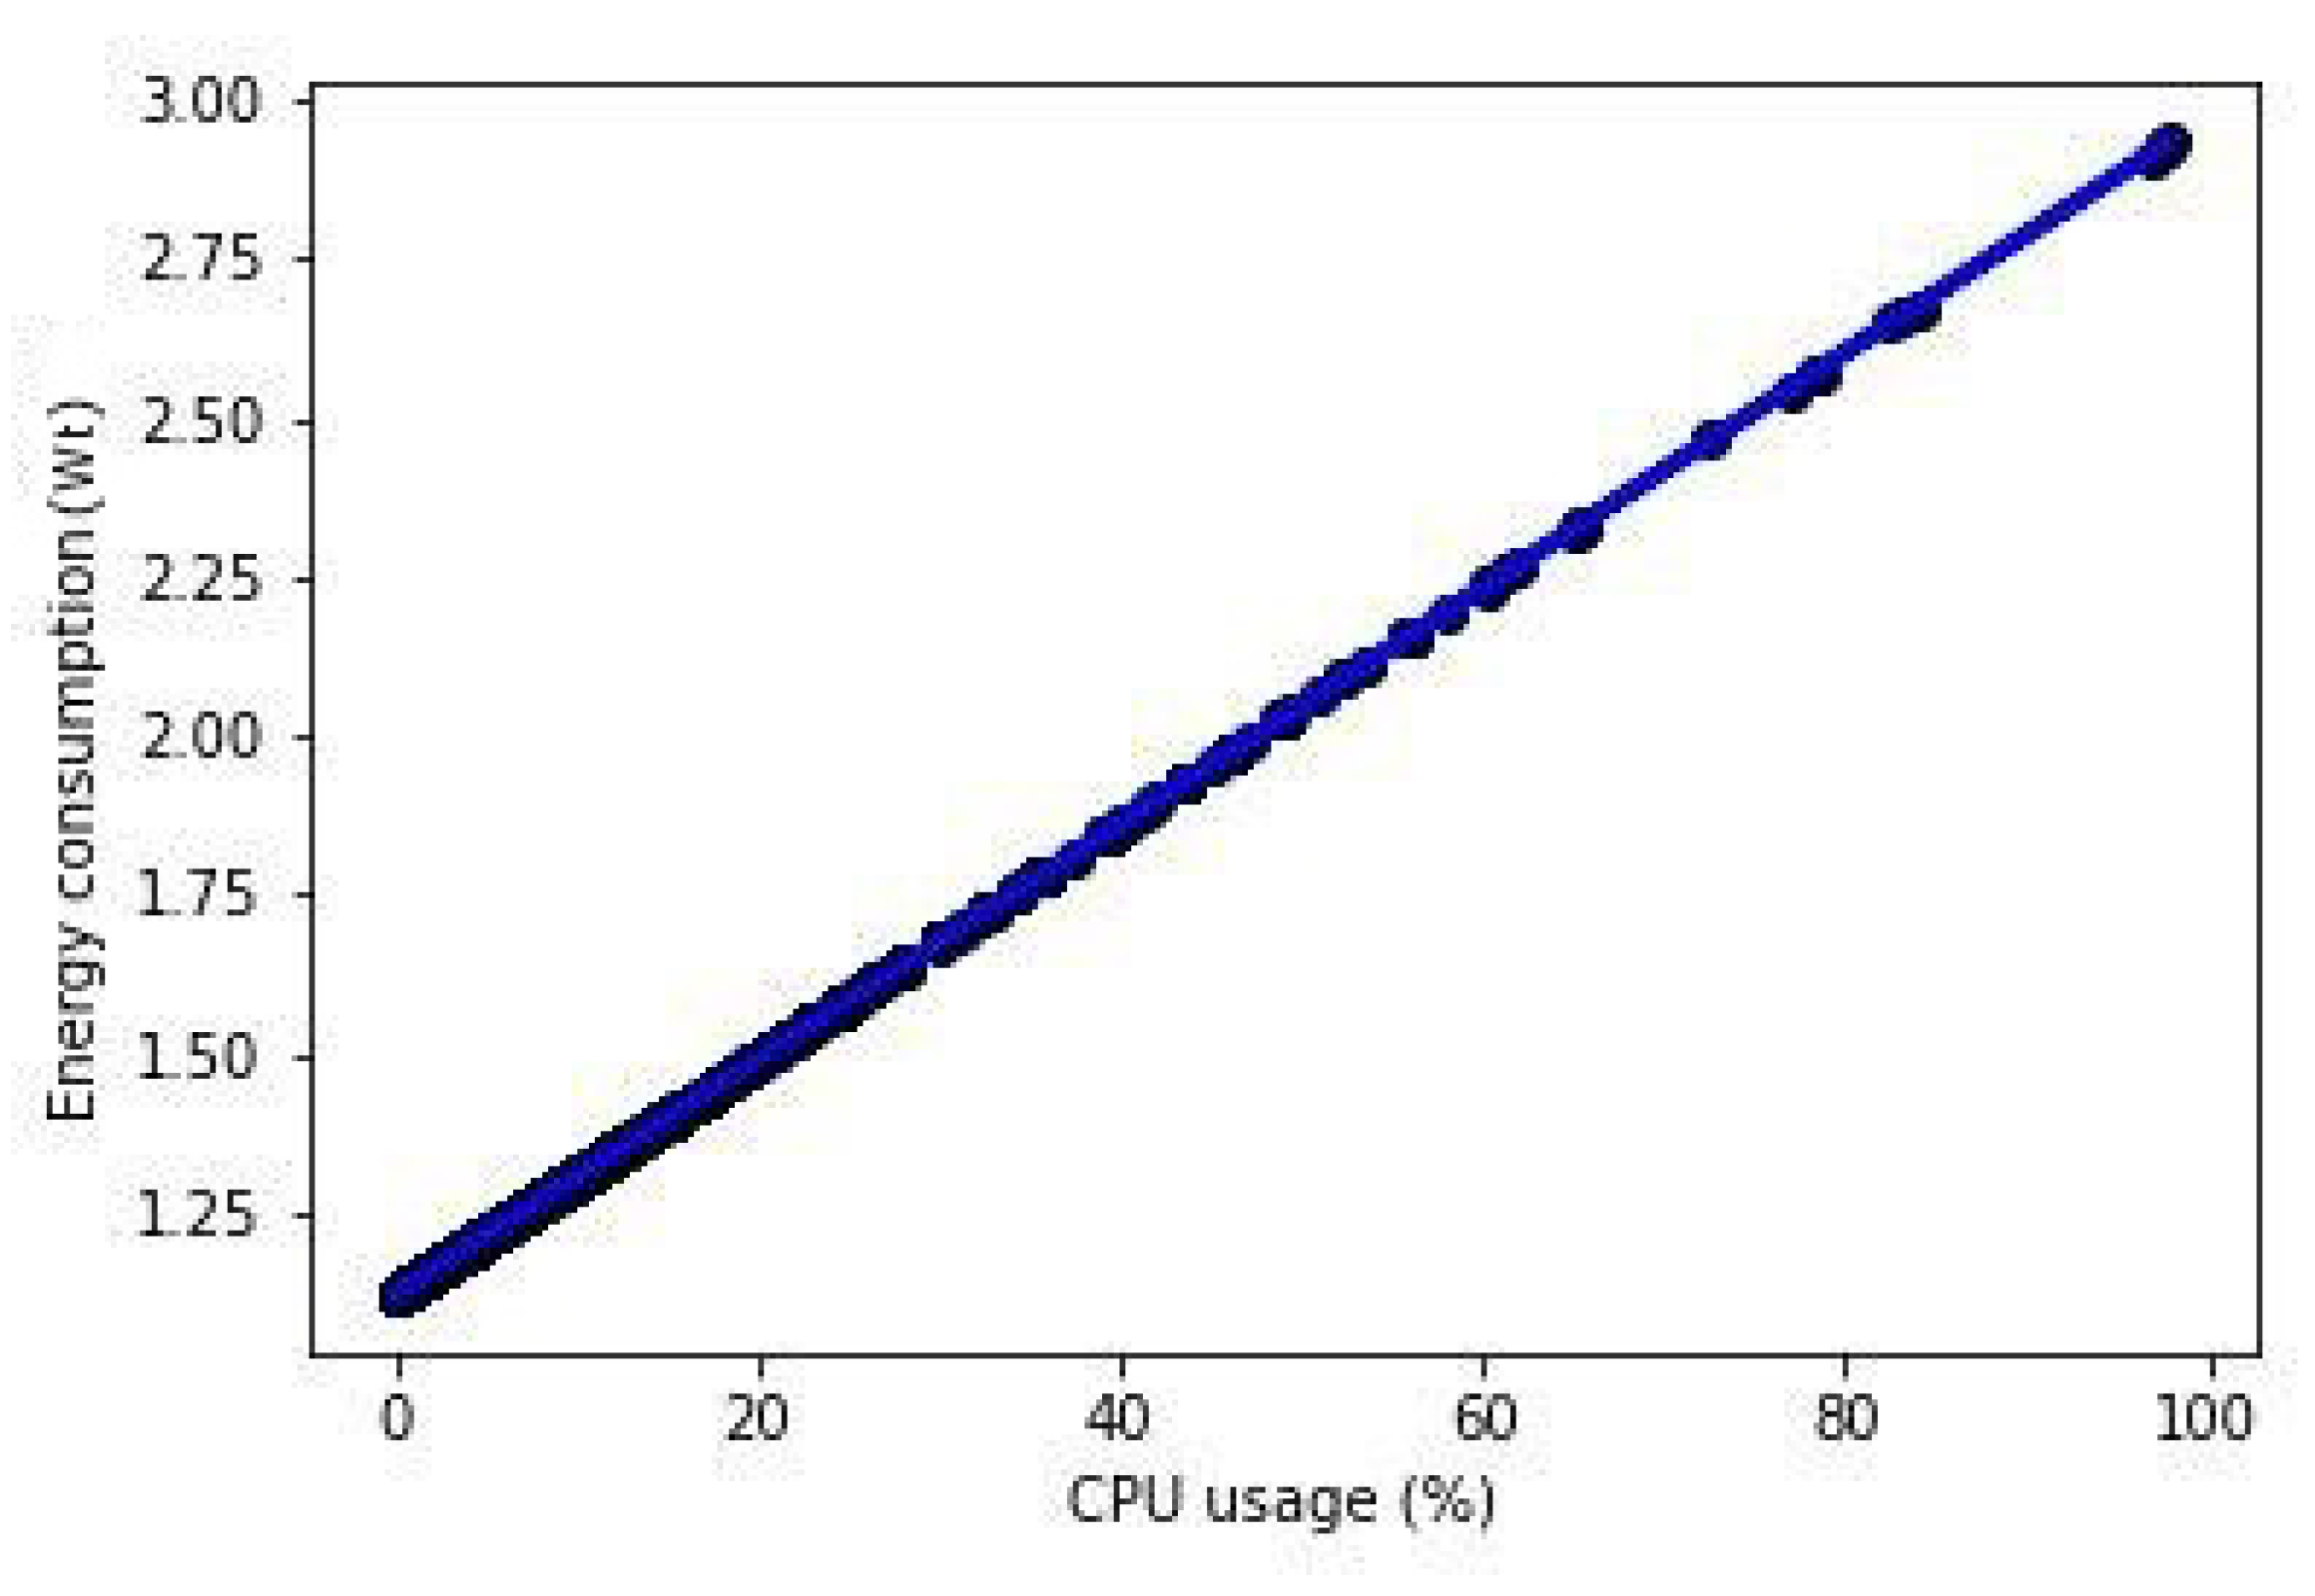
\includegraphics{cpu_usage_sota}
    \centering
    \caption{Representatie verbruik energie (Watt) tegenover CPU-gebruik (\%) \autocite{Ciancarini2020}}
    \label{cpu_usage_sota}
\end{figure}

\subsection{Meten van energieverbruik}
Het meten van energieverbruik bij software is een complexe taak. Volgens het onderzoek van \autocite{Dutta2023} is het echter niet de software dat energie verbruikt, maar is het de logica van de gecompileerde code die de hardware componenten, zoals de processor en geheugen, aanstuurt die op hun beurt energie verbruiken. Daarom refereert men vaak bij het vermelden van `energieverbruik van software` naar het energieverbruik van de hardware componenten die aangestuurd zijn door de code.\\

Twee vaak gebruikte manieren om het energieverbruik te meten van software zijn het gebruik van een energiemeter of een  proces op een Linux systeem die toelaten om het verbruik softwarematig te meten. Dit soort software maakt gebruik van  de RAPL technologie. RAPL, de afkorting voor ´Running Average Power Limit´, is een interface dat het actuele energie verbruik meet van een applicatie \autocite{Agarwal2023}. Een voorbeeld van software die deze technologie gebruikt is PowerJoular\footnote{https://github.com/joular/powerjoular}. Deze meet het verbruik van CPU en GPU van één of meerdere processen\autocite{Noureddine2022}. Voor andere operating systems blijkt het niet of moeilijk haalbaar om softwarematig energieverbruik te meten van applicaties. \\

Het meten via een energiemeter heeft als nadeel dat je niet op applicatie- of procesniveau kunt monitoren. Het meet namelijk de stroom dat direct uit het stopcontact verbruikt wordt. Hiermee kan dus wel het totale verbruik van het systeem gemonitord worden. Voor het meten op applicatieniveau kan er eerst een meting gebeuren op een idle systeem, waar het programma niet aan het runnen is, en dan een meting wanneer de applicatie wel actief is. Het verschil is dan het energieverbruik op applicatieniveau, alhoewel dit niet nauwkeurig is omdat eventuele andere achtergrondprocessen geactiveerd of gedeactiveerd kunnen worden tijdens de meting. \\

Het softwarematig meten van energieverbruik laat wel toe om op applicatie- of procesniveau te monitoren. Hiervoor is er een applicatie of proces nodig dat toegang heeft tot alle actieve processen op het systeem, alsook het resourcegebruik hiervan. Afhankelijk van de hardware kan de applicatie al dan niet rechtstreeks ook het energieverbruik tonen. \\
%https://github.com/joular/powerjoular


\subsection{Samengevat}
Energieverbruik van software is op meerdere vlakken al grondig onderzocht. Zo is er een verschil bij de keuze in programmeertaal. Kiezen voor de meest efficiënte compiled language kan tot wel 80 keer zo energiezuiniger werken dan de minst efficiënte interpreted language. Ook het hanteren van bepaalde programmeerprincipes zoals stijl of datatypes beïnvloeden het energieverbruik. Ook wijzen onderzoeken uit dat de compiler die de code uitvoert een degelijke impact heeft.\\

Verder is performantie ook een belangrijke factor. Inefficiënt gebruik van resources leidt tot hoger energieverbruik van componenten zoals CPU, RAM, disk, ... Om het verbruik van software in kaart te brengen kan men gebruik maken van een energiemeter of bepaalde software. Een energiemeter zal minder nauwkeurige resultaten afleveren dan de softwarematige metingen, maar kan in elke situatie gebruikt worden terwijl de softwarematige metingen vaak beperkt zijn tot 1 operating system. 

\section{Literatuurstudie samengevat}
De literatuurstudie richt zich op twee belangrijke aspecten: ontwikkelarchitecturen en energie-efficiëntie, of verschil in energieverbruik, van software. Ontwikkelarchitecturen bieden richtlijnen voor het ontwerp van softwareapplicaties, waarbij de structuur invloed heeft op prestaties, beveiliging, uitbreidbaarheid en kwaliteit. De vier bouwdelen van een architectuur zorgen voor een logische en toegankelijke opbouw die voldoet aan kwaliteitseisen en, in sommige gevallen, gemakkelijk uitbreidbaar is.\\

Het energieverbruik van software is uitgebreid onderzocht, met nadruk op verschillende aspecten die van invloed kunnen zijn. Bijvoorbeeld, de keuze van programmeertaal kan aanzienlijke verschillen in energieverbruik veroorzaken, waarbij compiled languages tot 80 keer energiezuiniger kunnen zijn dan interpreted languages. Programmeerprincipes zoals stijl en datatypes spelen ook een rol, evenals de compiler die de code uitvoert. Bovendien is het correct gebruiken van resources een cruciale factor, waarbij het niet optimaal gebruiken van resources leidt tot hoger energieverbruik van componenten zoals CPU, RAM en disk.\\

Om het energieverbruik van software in kaart te brengen, kunnen energiemeters of specifieke software worden gebruikt. Hoewel energiemeters minder nauwkeurige resultaten opleveren dan softwarematige metingen, zijn ze breed inzetbaar. Aan de andere kant zijn softwarematige metingen vaak beperkt tot één besturingssysteem.\\


% Tip: Begin elk hoofdstuk met een paragraaf inleiding die beschrijft hoe
% dit hoofdstuk past binnen het geheel van de bachelorproef. Geef in het
% bijzonder aan wat de link is met het vorige en volgende hoofdstuk.

% Pas na deze inleidende paragraaf komt de eerste sectiehoofding.

%Dit hoofdstuk bevat je literatuurstudie. De inhoud gaat verder op de inleiding, maar zal het onderwerp van de bachelorproef *diepgaand* uitspitten. De bedoeling is dat de lezer na lezing van dit hoofdstuk helemaal op de hoogte is van de huidige stand van zaken (state-of-the-art) in het onderzoeksdomein. Iemand die niet vertrouwd is met het onderwerp, weet nu voldoende om de rest van het verhaal te kunnen volgen, zonder dat die er nog andere informatie moet over opzoeken \autocite{Pollefliet2011}.

%Je verwijst bij elke bewering die je doet, vakterm die je introduceert, enz.\ naar je bronnen. In \LaTeX{} kan dat met het commando \texttt{$\backslash${textcite\{\}}} of \texttt{$\backslash${autocite\{\}}}. Als argument van het commando geef je de ``sleutel'' van een ``record'' in een bibliografische databank in het Bib\LaTeX{}-formaat (een tekstbestand). Als je expliciet naar de auteur verwijst in de zin (narratieve referentie), gebruik je \texttt{$\backslash${}textcite\{\}}. Soms is de auteursnaam niet expliciet een onderdeel van de zin, dan gebruik je \texttt{$\backslash${}autocite\{\}} (referentie tussen haakjes). Dit gebruik je bv.~bij een citaat, of om in het bijschrift van een overgenomen afbeelding, broncode, tabel, enz. te verwijzen naar de bron. In de volgende paragraaf een voorbeeld van elk.

%\textcite{Knuth1998} schreef een van de standaardwerken over sorteer- en zoekalgoritmen. Experten zijn het erover eens dat cloud computing een interessante opportuniteit vormen, zowel voor gebruikers als voor dienstverleners op vlak van informatietechnologie~\autocite{Creeger2009}.

%Let er ook op: het \texttt{cite}-commando voor de punt, dus binnen de zin. Je verwijst meteen naar een bron in de eerste zin die erop gebaseerd is, dus niet pas op het einde van een paragraaf.

%\lipsum[7-20]

%%=============================================================================
%% Methodologie
%%=============================================================================

\chapter{\IfLanguageName{dutch}{Methodologie}{Methodology}}%
\label{ch:methodologie}

%% TODO: In dit hoofstuk geef je een korte toelichting over hoe je te werk bent
%% gegaan. Verdeel je onderzoek in grote fasen, en licht in elke fase toe wat
%% de doelstelling was, welke deliverables daar uit gekomen zijn, en welke
%% onderzoeksmethoden je daarbij toegepast hebt. Verantwoord waarom je
%% op deze manier te werk gegaan bent.
%% 
%% Voorbeelden van zulke fasen zijn: literatuurstudie, opstellen van een
%% requirements-analyse, opstellen long-list (bij vergelijkende studie),
%% selectie van geschikte tools (bij vergelijkende studie, "short-list"),
%% opzetten testopstelling/PoC, uitvoeren testen en verzamelen
%% van resultaten, analyse van resultaten, ...
%%
%% !!!!! LET OP !!!!!
%%
%% Het is uitdrukkelijk NIET de bedoeling dat je het grootste deel van de corpus
%% van je bachelorproef in dit hoofstuk verwerkt! Dit hoofdstuk is eerder een
%% kort overzicht van je plan van aanpak.
%%
%% Maak voor elke fase (behalve het literatuuronderzoek) een NIEUW HOOFDSTUK aan
%% en geef het een gepaste titel.
%todo HERSCHRIJVEN!!!!!
\section{Literatuurstudie}
In deze fase is uitgebreid literatuuronderzoek uitgevoerd om inzicht te krijgen in de bestaande kennis en technologieën met betrekking tot het onderwerp van de bachelorproef, zijnde het energieverbruik van ontwikkelarchitecturen. Dit omvatte het bestuderen van relevante wetenschappelijke artikelen, boeken en online bronnen om een stevige basis van begrip op te bouwen.


\section{Short list}
Op basis van de literatuurstudie is een short list samengesteld van potentiële methoden, technologieën of tools die relevant zijn voor het onderzoek en gebruikt kunnen worden in de Proof of Concept. Deze selectie is gebaseerd op criteria zoals relevantie, toepasbaarheid, en beschikbaarheid van middelen.


\section{Opzetten PoC}
Na het vaststellen van de short list is een Proof of Concept (PoC) opgezet. Dit omvatte het ontwerpen en implementeren van een applicatie binnen verschillende architecturen.


\section{Uitvoeren testen op PoC}
Met de PoC opgezet, werden gestructureerde tests uitgevoerd om het energieverbruik per architectuur te beoordelen. Hierbij zijn diverse metingen en observaties gedaan om data te verzamelen.


\section{Analyse van testresultaten}
De verzamelde data uit de tests op de PoC zijn geanalyseerd om inzicht te krijgen in de energie-efficiëntie van de verschillende architecturen. 

\section{Conclusie}
Op basis van de uitgevoerde tests en de analyse van de resultaten worden conclusies getrokken met betrekking tot de geschiktheid en toepasbaarheid van de onderzochte methoden of technologieën. Ook worden eventuele suggesties voor toekomstig onderzoek of verbeteringen aangedragen.


% Voeg hier je eigen hoofdstukken toe die de ``corpus'' van je bachelorproef
% vormen. De structuur en titels hangen af van je eigen onderzoek. Je kan bv.
% elke fase in je onderzoek in een apart hoofdstuk bespreken.

%\input{...}
%\input{...}
%...

%%=============================================================================
%% Conclusie
%%=============================================================================

\chapter{Conclusie}%
\label{ch:conclusie}

% TODO: Trek een duidelijke conclusie, in de vorm van een antwoord op de
% onderzoeksvra(a)g(en). Wat was jouw bijdrage aan het onderzoeksdomein en
% hoe biedt dit meerwaarde aan het vakgebied/doelgroep? 
% Reflecteer kritisch over het resultaat. In Engelse teksten wordt deze sectie
% ``Discussion'' genoemd. Had je deze uitkomst verwacht? Zijn er zaken die nog
% niet duidelijk zijn?
% Heeft het onderzoek geleid tot nieuwe vragen die uitnodigen tot verder 
%onderzoek?

Dit onderzoek richtte zich op het analyseren van de impact van architecturale veranderingen op het energieverbruik van een applicatie, specifiek door het vergelijken van een monolithische architectuur met een microservice architectuur. De centrale onderzoeksvraag was: "Wat is de impact op energieverbruik bij een architecturale verandering van een applicatie?".\\

Uit de literatuurstudie bleek dat de gekozen ontwikkelarchitectuur aanzienlijke invloed heeft op de prestaties en het energieverbruik van een applicatie. Ontwikkelarchitecturen bieden richtlijnen voor het structureren van een applicatie, waardoor deze uitbreidbaar, logisch opgebouwd en kwalitatief hoogstaand blijft. Bovendien speelt de keuze van programmeertaal en programmeerprincipes een cruciale rol bij het optimaliseren van energieverbruik.\\

De uitgewerkte Proof of Concept (PoC) applicatie bestaat uit een monolithische en een microservice versie. Beide versies, gehost in een docker omgeving, bevatten specifieke methoden en controllers om gebruikers te laten inloggen en het verbruik van telefoonnummers te raadplegen. Zo zijn zowel resource intensieve als niet resource intensieve functies gesimuleerd in de applicatie.\\

De uitgevoerde tests onderwierpen beide architecturen aan een groot aantal requests om het energieverbruik te meten. Hierbij werd gebruik gemaakt van softwarematige metingen, meer bepaald de RAPL technologie, om de energieconsumptie nauwkeurig in kaart te brengen.\\

Uit de resultaten kan geconcludeerd worden dat een verandering in ontwikkelarchitectuur een degelijke impact kan hebben op het energieverbruik van de applicatie. Alhoewel de microservice langer gemiddeld een lager energieverbruik heeft per scenario, duurt het langer om dezelfde scenario's uit te voeren dan op de monoliet, waardoor een groter totaal verbruik is. Dit komt doordat de microservice applicatie afhankelijk is van de API responstijd, terwijl de monoliet applicatie een inkomende web request direct kan verwerken zonder afhankelijk te zijn van een externe service. Dit onderzoek duidt verder aan dat een microservice architectuur niet de beste optie is om het energieverbruik van een applicatie te verminderen. Als conclusie kan dus gesteld worden dat een architecturale wijziging van applicatie een negatieve impact kan hebben op het energieverbruik. Deze bevindingen zijn relevant voor ontwikkelaars en bedrijven die op zoek zijn naar een manier om  het energieverbruik bij hun softwareontwikkeling te verminderen.\\

In toekomstige onderzoeken zou men verder kunnen ingegaan op andere software ontwikkelarchitecturen zoals de serverless of event driven architectuur. Door de impact op energieverbruik van deze andere ontwikkelarchitecturen te onderzoeken, kan een beter beeld gevormd worden in hoe softwareontwikkelaars en bedrijven hun systemen kunnen optimaliseren voor zowel prestaties als duurzaamheid. Deze bevindingen kunnen bijdragen aan meer geïnformeerde beslissingen over architecturale keuzes en hun implicaties voor energieverbruik.

%---------- Bijlagen -----------------------------------------------------------

\appendix

\chapter{Onderzoeksvoorstel}

Het onderwerp van deze bachelorproef is gebaseerd op een onderzoeksvoorstel dat vooraf werd beoordeeld door de promotor. Dat voorstel is opgenomen in deze bijlage.

%% TODO: 
%\section*{Samenvatting}

% Kopieer en plak hier de samenvatting (abstract) van je onderzoeksvoorstel.

% Verwijzing naar het bestand met de inhoud van het onderzoeksvoorstel
%---------- Inleiding ---------------------------------------------------------

\section{Introductie}%
\label{sec:introductie}
Deze bachelorproef onderzoekt de mogelijke voordelen en uitdagingen in het migreren van een bestaande PHP-webapplicatie naar het ASP.NET framework. Davo Group NV heeft een bestaande web applicatie gebouwd in PHP, maar stellen zich de vraag of een migratie naar ASP.NET een effectievere server-side oplossing zou zijn. De doelgroep van deze bachelorproef zijn de ontwikkelaars binnen Davo Group NV die verantwoordelijk zijn voor de evolutie van de bestaande PHP-webapplicatie.

Het thema gaat concreet over de keuze van server-side frameworks, waarbij er gefocust wordt op het verschil tussen PHP en ASP.NET. Het probleem is namelijk dat er een optimaal server-side framework gevonden moet worden om de huidige PHP-applicatie mogelijks te vervangen. We richten ons specifiek op de technische en prestatiegerelateerde aspecten om de impact op performantie, security en ontwikkeltijd in kaart te brengen. 

De vraag die heerst in deze bachelorproef is of een migratie van de PHP-webapplicatie naar ASP.NET een positieve impact zal hebben.
De bedoeling is om 2 resultaten te verkrijgen. Het eerste resultaat is een grondige analyse van de technische aspecten van PHP en ASP.NET. Het andere resultaat is een aanbeveling of de migratie naar ASP.NET een effectievere oplossing is dan de huidige PHP-webapplicatie.


%
%Waarover zal je bachelorproef gaan? Introduceer het thema en zorg dat volgende zaken zeker duidelijk aanwezig zijn:
%
%\begin{itemize}
%  \item kaderen thema
%  \item de doelgroep
%  \item de probleemstelling en (centrale) onderzoeksvraag
%  \item de onderzoeksdoelstelling
%\end{itemize}
%
%Denk er aan: een typische bachelorproef is \textit{toegepast onderzoek}, wat betekent dat je start vanuit een concrete probleemsituatie in bedrijfscontext, een \textbf{casus}. Het is belangrijk om je onderwerp goed af te bakenen: je gaat voor die \textit{ene specifieke probleemsituatie} op zoek naar een goede oplossing, op basis van de huidige kennis in het vakgebied.
%
%De doelgroep moet ook concreet en duidelijk zijn, dus geen algemene of vaag gedefinieerde groepen zoals \emph{bedrijven}, \emph{developers}, \emph{Vlamingen}, enz. Je richt je in elk geval op it-professionals, een bachelorproef is geen populariserende tekst. Eén specifiek bedrijf (die te maken hebben met een concrete probleemsituatie) is dus beter dan \emph{bedrijven} in het algemeen.
%
%Formuleer duidelijk de onderzoeksvraag! De begeleiders lezen nog steeds te veel voorstellen waarin we geen onderzoeksvraag terugvinden.
%
%Schrijf ook iets over de doelstelling. Wat zie je als het concrete eindresultaat van je onderzoek, naast de uitgeschreven scriptie? Is het een proof-of-concept, een rapport met aanbevelingen, \ldots Met welk eindresultaat kan je je bachelorproef als een succes beschouwen?

%---------- Stand van zaken ---------------------------------------------------

\section{State-of-the-art}%
\label{sec:state-of-the-art}
\subsection{Wat is php?}
\subsubsection{Definitie}
\subsubsection{Voor- en nadelen}
\subsection{Wat is ASP.NET?}
\subsubsection{Definitie}
\subsubsection{Voor- en nadelen}


%Hier beschrijf je de \emph{state-of-the-art} rondom je gekozen onderzoeksdomein, d.w.z.\ een inleidende, doorlopende tekst over het onderzoeksdomein van je bachelorproef. Je steunt daarbij heel sterk op de professionele \emph{vakliteratuur}, en niet zozeer op populariserende teksten voor een breed publiek. Wat is de huidige stand van zaken in dit domein, en wat zijn nog eventuele open vragen (die misschien de aanleiding waren tot je onderzoeksvraag!)?
%
%Je mag de titel van deze sectie ook aanpassen (literatuurstudie, stand van zaken, enz.). Zijn er al gelijkaardige onderzoeken gevoerd? Wat concluderen ze? Wat is het verschil met jouw onderzoek?
%
%Verwijs bij elke introductie van een term of bewering over het domein naar de vakliteratuur, bijvoorbeeld~\autocite{Hykes2013}! Denk zeker goed na welke werken je refereert en waarom.
%
%Draag zorg voor correcte literatuurverwijzingen! Een bronvermelding hoort thuis \emph{binnen} de zin waar je je op die bron baseert, dus niet er buiten! Maak meteen een verwijzing als je gebruik maakt van een bron. Doe dit dus \emph{niet} aan het einde van een lange paragraaf. Baseer nooit teveel aansluitende tekst op eenzelfde bron.
%
%Als je informatie over bronnen verzamelt in JabRef, zorg er dan voor dat alle nodige info aanwezig is om de bron terug te vinden (zoals uitvoerig besproken in de lessen Research Methods).

% Voor literatuurverwijzingen zijn er twee belangrijke commando's:
% \autocite{KEY} => (Auteur, jaartal) Gebruik dit als de naam van de auteur
%   geen onderdeel is van de zin.
% \textcite{KEY} => Auteur (jaartal)  Gebruik dit als de auteursnaam wel een
%   functie heeft in de zin (bv. ``Uit onderzoek door Doll & Hill (1954) bleek
%   ...'')

%Je mag deze sectie nog verder onderverdelen in subsecties als dit de structuur van de tekst kan verduidelijken.

%---------- Methodologie ------------------------------------------------------
\section{Methodologie}%
\label{sec:methodologie}

Hier beschrijf je hoe je van plan bent het onderzoek te voeren. Welke onderzoekstechniek ga je toepassen om elk van je onderzoeksvragen te beantwoorden? Gebruik je hiervoor literatuurstudie, interviews met belanghebbenden (bv.~voor requirements-analyse), experimenten, simulaties, vergelijkende studie, risico-analyse, PoC, \ldots?

Valt je onderwerp onder één van de typische soorten bachelorproeven die besproken zijn in de lessen Research Methods (bv.\ vergelijkende studie of risico-analyse)? Zorg er dan ook voor dat we duidelijk de verschillende stappen terug vinden die we verwachten in dit soort onderzoek!

Vermijd onderzoekstechnieken die geen objectieve, meetbare resultaten kunnen opleveren. Enquêtes, bijvoorbeeld, zijn voor een bachelorproef informatica meestal \textbf{niet geschikt}. De antwoorden zijn eerder meningen dan feiten en in de praktijk blijkt het ook bijzonder moeilijk om voldoende respondenten te vinden. Studenten die een enquête willen voeren, hebben meestal ook geen goede definitie van de populatie, waardoor ook niet kan aangetoond worden dat eventuele resultaten representatief zijn.

Uit dit onderdeel moet duidelijk naar voor komen dat je bachelorproef ook technisch voldoen\-de diepgang zal bevatten. Het zou niet kloppen als een bachelorproef informatica ook door bv.\ een student marketing zou kunnen uitgevoerd worden.

Je beschrijft ook al welke tools (hardware, software, diensten, \ldots) je denkt hiervoor te gebruiken of te ontwikkelen.

Probeer ook een tijdschatting te maken. Hoe lang zal je met elke fase van je onderzoek bezig zijn en wat zijn de concrete \emph{deliverables} in elke fase?

%---------- Verwachte resultaten ----------------------------------------------
\section{Verwacht resultaat, conclusie}%
\label{sec:verwachte_resultaten}

Hier beschrijf je welke resultaten je verwacht. Als je metingen en simulaties uitvoert, kan je hier al mock-ups maken van de grafieken samen met de verwachte conclusies. Benoem zeker al je assen en de onderdelen van de grafiek die je gaat gebruiken. Dit zorgt ervoor dat je concreet weet welk soort data je moet verzamelen en hoe je die moet meten.

Wat heeft de doelgroep van je onderzoek aan het resultaat? Op welke manier zorgt jouw bachelorproef voor een meerwaarde?

Hier beschrijf je wat je verwacht uit je onderzoek, met de motivatie waarom. Het is \textbf{niet} erg indien uit je onderzoek andere resultaten en conclusies vloeien dan dat je hier beschrijft: het is dan juist interessant om te onderzoeken waarom jouw hypothesen niet overeenkomen met de resultaten.



%%---------- Andere bijlagen --------------------------------------------------
% TODO: Voeg hier eventuele andere bijlagen toe. Bv. als je deze BP voor de
% tweede keer indient, een overzicht van de verbeteringen t.o.v. het origineel.
%\input{...}

%%---------- Backmatter, referentielijst ---------------------------------------

\backmatter{}

\setlength\bibitemsep{2pt} %% Add Some space between the bibliograpy entries
\printbibliography[heading=bibintoc]

\end{document}
